\documentclass{siamart1116}
\usepackage{amsmath, amssymb}
%\usepackage{amsmath,amssymb,amsfonts,graphicx,amsthm,dsfont}
%\usepackage{listings}
%\usepackage{courier}
\usepackage{enumerate}
%\usepackage{color}
%\usepackage[usenames,dvipsnames]{xcolor}
%\usepackage{hyperref,tikz,mdframed}
%\hypersetup{colorlinks=true,urlcolor=MidnightBlue,citecolor=PineGreen,linkcolor=BrickRed}

% \lstset{
% 	basicstyle=\small\ttfamily,
% 	keywordstyle=\color{blue},
% 	language=python,
% 	xleftmargin=16pt,
% }
\usepackage{algorithmicx}
\usepackage{algpseudocode}% http://ctan.org/pkg/algorithmicx
\usepackage{multicol}

\textwidth=5.8in
\textheight=9in
\topmargin=-0.5in
\headheight=0in
\headsep=.5in
\hoffset  -.4in
\pagestyle{empty}

\newcommand{\Fp}{\mathbb{F}_p}
\newcommand{\Q}{\mathbb{Q}}
\newcommand{\Z}{\mathbb{Z}}
\newcommand{\kron}[2]{\left(\frac{#1}{#2}\right)}
\newcommand{\Aut}{\mathrm{Aut}}
\newcommand{\End}{\mathrm{End}}
\newcommand{\SO}{\mathrm{SO}}
\newcommand{\SU}{\mathrm{SU}}
\newcommand{\tr}{\operatorname{tr}}
\newcommand{\dee}{\mathrm{d}}
\newcommand{\deee}{\textbf{\text{\emph{d}}}}

\newcommand{\md}[1]{\textcolor{cyan}{#1}}

\newcommand{\TheAuthors}{V. Chen}

%\newtheorem{theorem}{Theorem}
%\newtheorem{definition}{Definition}

\graphicspath{ {graphics/} }

\title{Week 2 Summary}
\author{\TheAuthors}
\date{}
\begin{document}
\maketitle
\setlength{\unitlength}{1in}
\setlength{\parindent}{0in}

\section{Summary}
Last week's experiments indicated that the original parameterization, treating $u, \tau, \alpha$ as the variables, would not converge even after 100,000 iterations. First, we explain the different parameterization that we tried this week. We decided to try a different parameterization which treats $\xi, \tau, \alpha$ as variables to sample, and we compare results between this and the old parameterization.

\section{Learning $\tau$ and $\alpha$ with non-centered parameterization}
\subsection{Algorithm}
In the centered parameterization, the prior was $u|\tau,\alpha \sim N(0, C(\tau, \alpha))$, $\tau, \alpha$ distributed independently and uniformly over intervals. We would take the posterior by Bayes' theorem to be
\[f(u,\tau,\alpha) \propto \exp\left(-\Phi(u) -\frac{1}{2}\langle u, C(\tau,\alpha)^{-1}u \rangle - \frac{1}{2}\log(\det(C(\tau,\alpha))) + \log(\pi_0(\tau,\alpha))\right) \]
In the new parameterization, we sample $\xi \sim N(0, I)$ and $\tau, \alpha$ on uniform intervals as before. $\xi$ is related to $u$ by $T(\xi,\tau,\alpha) = u = \sum_{j=0}^{M}(\lambda_j+\tau^2)^{-\alpha/2}\xi_jq_j$. Recall that we are taking $M=N-1$. The new joint posterior becomes:
\[ g(\xi,\tau,\alpha) \propto \exp\left( -\Phi(T(\xi,\tau,\alpha))-\frac{1}{2}\langle \xi,\xi \rangle + \log(\pi_0(\tau,\alpha)) \right)\]
This algorithm works as follows:
\begin{algorithm}
\caption{Non-centered parameterization: sampling $\xi, \tau, \alpha$}
\label{alg:xi_tau_alpha}
\begin{algorithmic}
\State Choose $\xi^{(0)} \in \mathbb{R}^N, \alpha^{(0)}, \tau^{(0)} > 0, \beta \in (0, 1]$ and $\epsilon_1, \epsilon_2 > 0$.
\For{$k=0$ to $S$}
\State Propose $\hat\xi^{(k)} = (1-\beta^2)\xi^{(k)} + \beta \zeta^{(k)}$, $\zeta^{(k)} \sim N(0, I)$
\State Make transition $\xi^{(k+1)} \to \hat\xi^{(k)}$ with probability
\[ A(\xi^{(k)} \to \hat\xi^{(k)}) = \min\{1, \frac{g(\hat\xi^{(k)},\tau^{(k)},\alpha^{(k)})}{g(\xi^{(k)},\tau^{(k)},\alpha^{(k)})} \}\]

\State Propose $\hat\tau^{(k)} = \tau^{(k)} + \epsilon_1 \rho^{(k)}, \rho^{(k)} \sim N(0,I)$
\State Make transition $\tau^{(k+1)} \to \hat\tau^{(k)}$ with probability
\[ A(\tau^{(k)} \to \hat\tau^{(k)}) = \min\{1, \frac{g(\xi^{(k+1)},\hat\tau^{(k)},\alpha^{(k)})}{g(\xi^{(k+1)},\tau^{(k)},\alpha^{(k)})} \}\]

\State Propose $\hat\alpha^{(k)} = \alpha^{(k)} + \epsilon_2 \sigma^{(k)}, \sigma^{(k)} \sim N(0,I)$
\State Make transition $\alpha^{(k+1)} \to \hat\alpha^{(k)}$ with probability
\[ A(\alpha^{(k)} \to \hat\alpha^{(k)}) = \min\{1, \frac{g(\xi^{(k+1)},\tau^{(k+1)},\hat \alpha^{(k)})}{g(\xi^{(k+1)},\tau^{(k+1)},\alpha^{(k)})} \}\]
\EndFor
\State \Return $\{ T(\xi^{(k)},\tau^{(k)},\alpha^{(k)}), \tau^{(k)}, \alpha^{k} \}$
\end{algorithmic}
\end{algorithm}

\subsection{Simulation results}
The relevant figures are \cref{fig:hier_sim_1}, \cref{fig:hier_sim_2}, \cref{fig:hier_sim_3}, \cref{fig:hier_sim_4}, \cref{fig:hier_sim_5}, \cref{fig:hier_sim_6}. The parameters used are as follows:
\begin{center}
\begin{tabular}{| c | c |}
\hline
Iterations & 100000 \\ \hline
Burn in period & 1000 \\ \hline
Laplacian & self-tuning, unnormalized \\ \hline
$\beta$ & $0.1$\\ \hline
$\gamma$ & $0.0001$\\ \hline
Labeled +1 & $280-290$ \\ \hline
Labeled -1 & $20-30$ \\ \hline
$\epsilon_\alpha$ & $1$\\ \hline
$\epsilon_\tau$ & $1$\\ \hline
Initial $\tau$ & $30$\\ \hline
Initial $\alpha$ & $5$\\ \hline
$\tau$ range & $[0, 60]$\\ \hline
$\alpha$ range & $[0, 100]$\\ \hline
Average $\tau$ & $3.74$\\ \hline
Average $\alpha$ & $63.5$\\ \hline
Percent of correct classification & $0.864407$ \\ \hline
Time elapsed & 183.21 s \\ \hline
\end{tabular}
\end{center}

\begin{figure}[!htb]
    \begin{minipage}{0.48\textwidth}
        \centering
        \caption{\label{fig:hier_sim_1} $\alpha$ acceptance probability}
        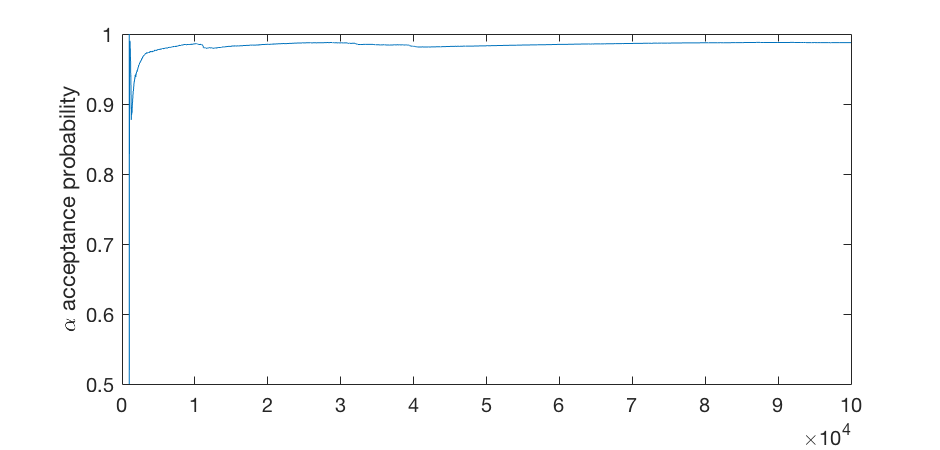
\includegraphics[width=\linewidth]{graphics/noncentered/acceptance_alpha_probability.png}
    \end{minipage} \hfill
    \begin{minipage}{0.48\textwidth}
        \centering
        \caption{\label{fig:hier_sim_2} $\alpha$ trace}
        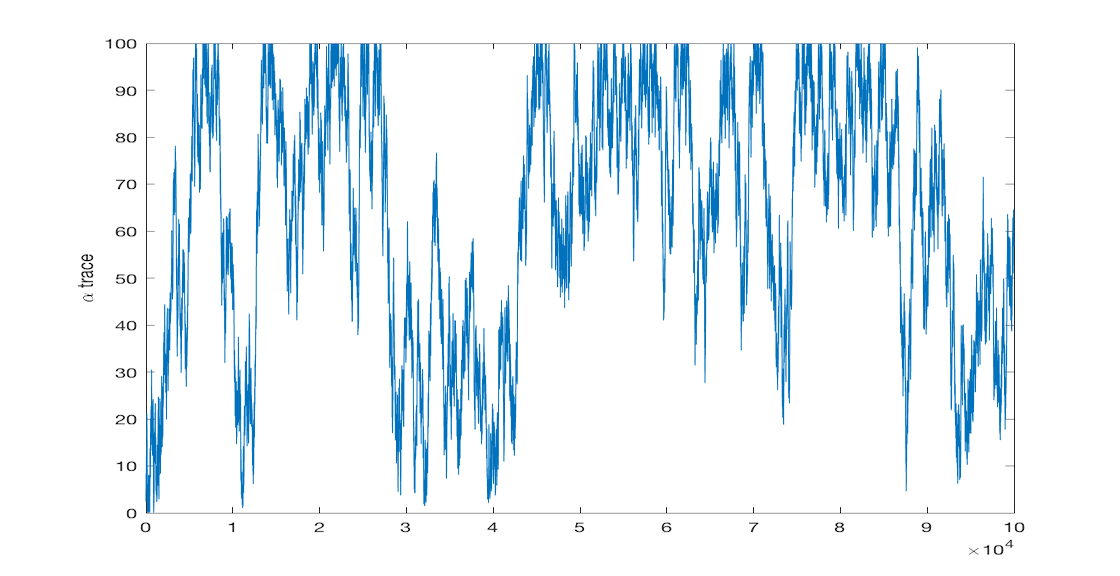
\includegraphics[width=\linewidth]{graphics/noncentered/trace_alpha.png}
    \end{minipage}
\end{figure}

\begin{figure}[!htb]
    \begin{minipage}{0.48\textwidth}
        \centering
        \caption{\label{fig:hier_sim_3} $\tau$ acceptance probability}
        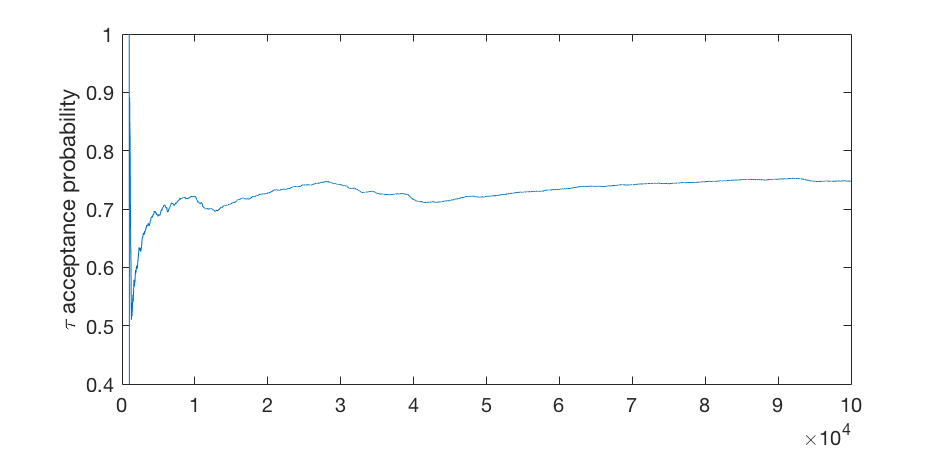
\includegraphics[width=\linewidth]{graphics/noncentered/acceptance_tau_probability.png}
    \end{minipage} \hfill
    \begin{minipage}{0.48\textwidth}
        \centering
        \caption{\label{fig:hier_sim_4}  $\tau$ trace}
        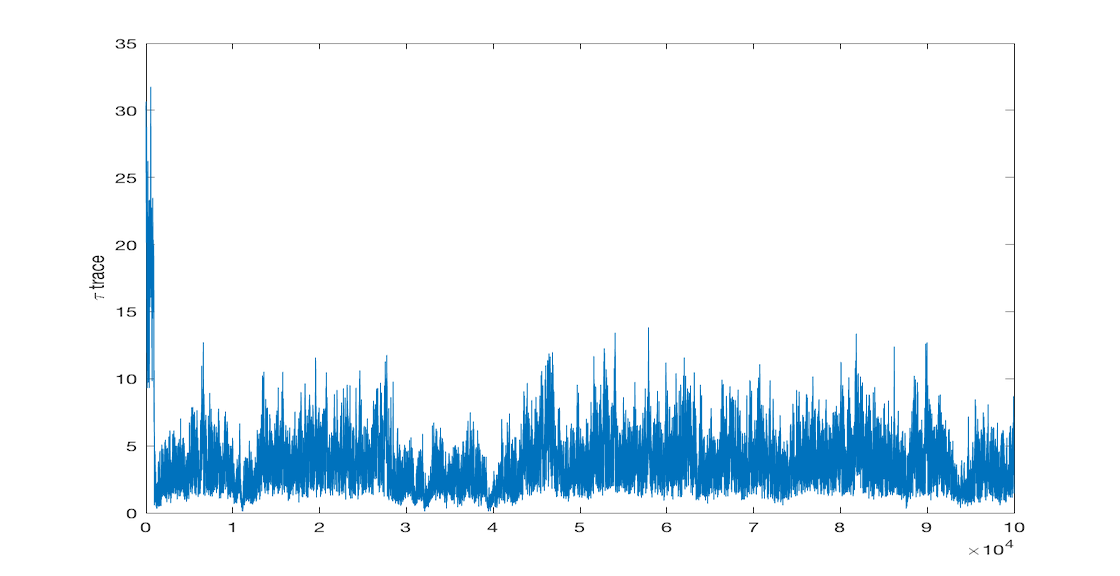
\includegraphics[width=\linewidth]{graphics/noncentered/trace_tau.png}
    \end{minipage}
\end{figure}

\begin{figure}[!htb]
    \begin{minipage}{0.48\textwidth}
        \centering
        \caption{\label{fig:hier_sim_5} $\xi$ acceptance probability}
        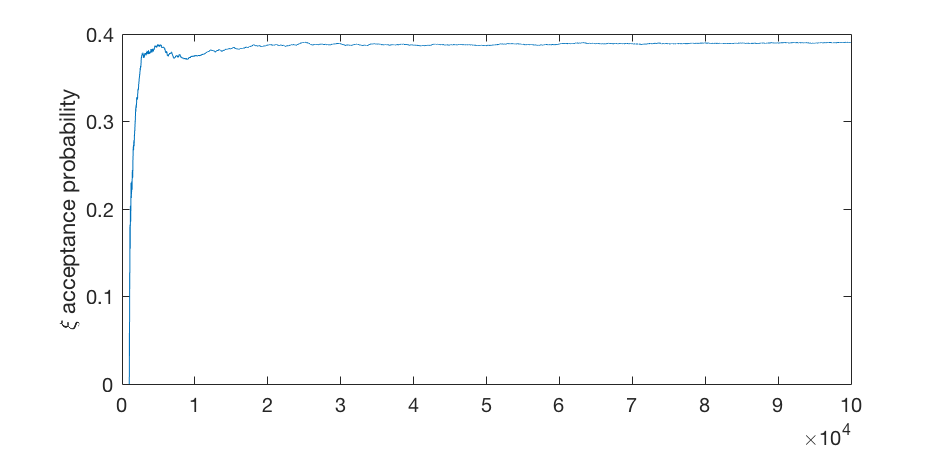
\includegraphics[width=\linewidth]{graphics/noncentered/acceptance_xi_probability.png}
    \end{minipage} \hfill
    \begin{minipage}{0.48\textwidth}
        \centering
        \caption{\label{fig:hier_sim_6} $u$ final average}
        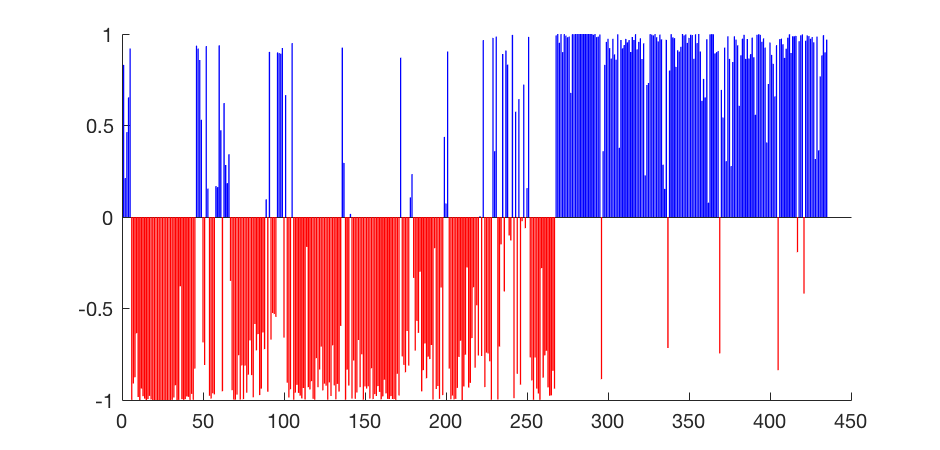
\includegraphics[width=\linewidth]{graphics/noncentered/final_avg.png}
    \end{minipage}
\end{figure}

\section{Revisiting the centered parameterization}
Matt took a look at my code and suggested that part of the reason why the parameters do not mix well is because of the accuracy of Matlab's eig solver for large eigenvalues, since the eigenvectors are very irregular. From Matt's suggestion, I truncated the sum after $M=50$ terms, a spectral projection. Applying this algorithm to the voting data set, the average $u$ was able to quickly converge to a function similar to the Fiedler vector, and the hyperparameters $\tau$ and $\alpha$ showed better mixing.
\begin{center}
\begin{tabular}{| c | c |}
\hline
Laplacian & self-tuning, unnormalized \\ \hline
$\beta$ & $0.4$\\ \hline
$\gamma$ & $0.0001$\\ \hline
Labeled +1 & $280-290$ \\ \hline
Labeled -1 & $20-30$ \\ \hline
$\epsilon_\alpha$ & $0.1$\\ \hline
$\epsilon_\tau$ & $1$\\ \hline
Initial $\tau$ & $20$\\ \hline
Initial $\alpha$ & $20$\\ \hline
Percent of correct classification & $0.837772$ \\ \hline
\end{tabular}
\end{center}
\begin{figure}[!htb]
    \begin{minipage}{0.48\textwidth}
        \centering
        \caption{\label{fig:centered_truncated_tau} $\tau$ trace}
        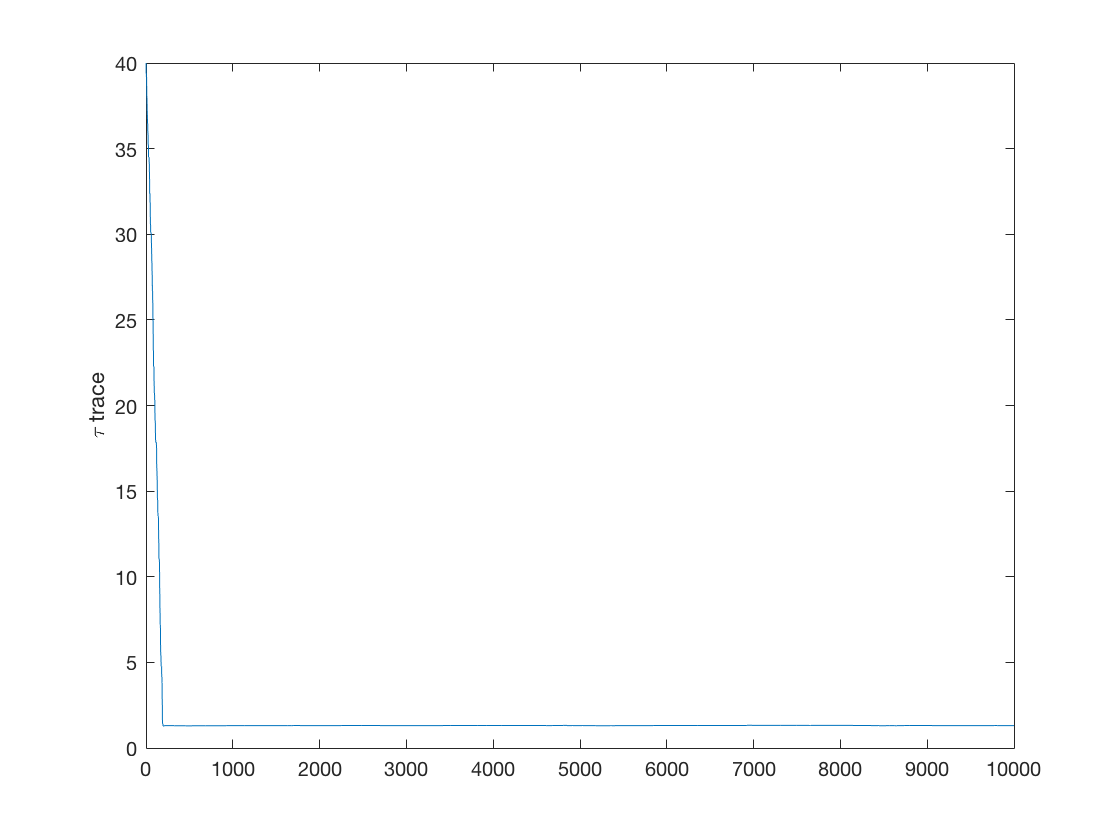
\includegraphics[width=\linewidth]{graphics/centered/trace_tau.png}
    \end{minipage} \hfill
    \begin{minipage}{0.48\textwidth}
        \centering
        \caption{\label{fig:centered_truncated_alpha} $\alpha$ trace}
        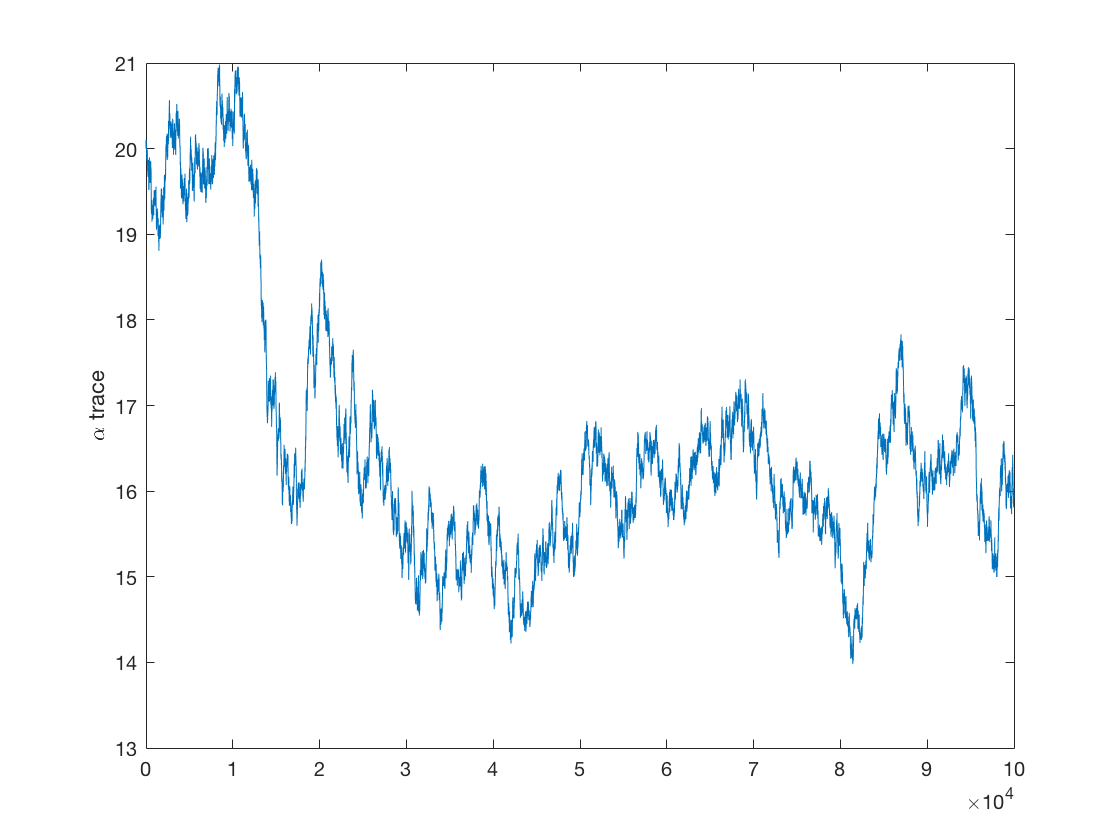
\includegraphics[width=\linewidth]{graphics/centered/trace_alpha.png}
    \end{minipage}
\end{figure}

\section{Two moons data}
We began to test our algorithms on the two moons data. We used $1000$ nodes and noise in $100$ dimensions with standard deviation $\sigma = 0.1$. We labeled about $4\%$ of the nodes.
\subsection{Centered parameterization}
The centered parameterization with the unnormalized Laplacian and without truncation does not perform well on the two moons data set. This could again be due to higher order eigenvectors. See \cref{fig:moon_untruncated_tau}, \cref{fig:moon_untruncated_alpha}, \cref{fig:moon_untruncated_avg}, \cref{fig:moon_untruncated_scatter}.

\begin{figure}[!htb]
    \begin{minipage}{0.48\textwidth}
        \centering
        \caption{\label{fig:moon_untruncated_tau} Without truncation, $\tau$ trace}
        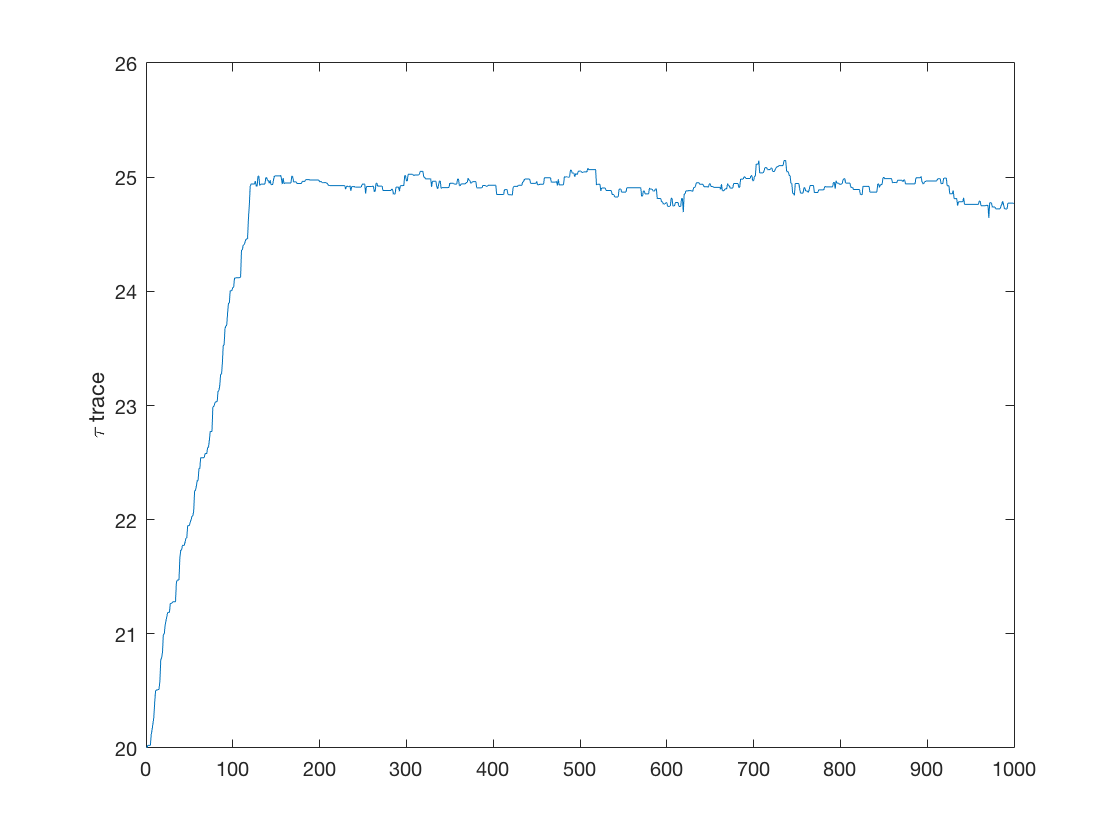
\includegraphics[width=\linewidth]{graphics/moons/centered_untruncated/trace_tau.png}
    \end{minipage} \hfill
    \begin{minipage}{0.48\textwidth}
        \centering
        \caption{\label{fig:moon_untruncated_alpha} Without truncation, $\alpha$ trace}
        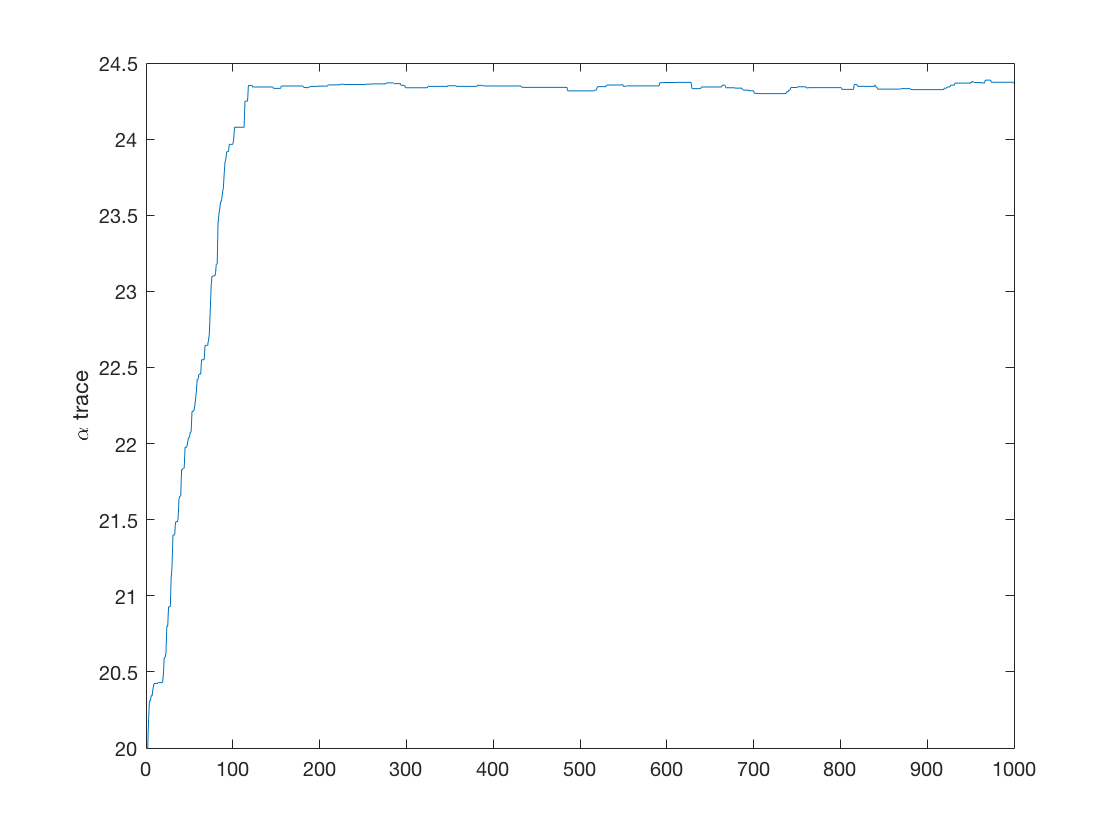
\includegraphics[width=\linewidth]{graphics/moons/centered_untruncated/trace_alpha.png}
    \end{minipage}
\end{figure}
\begin{figure}[!htb]
    \begin{minipage}{0.48\textwidth}
        \centering
        \caption{\label{fig:moon_untruncated_avg} Without truncation, average eigenfunction $u$}
        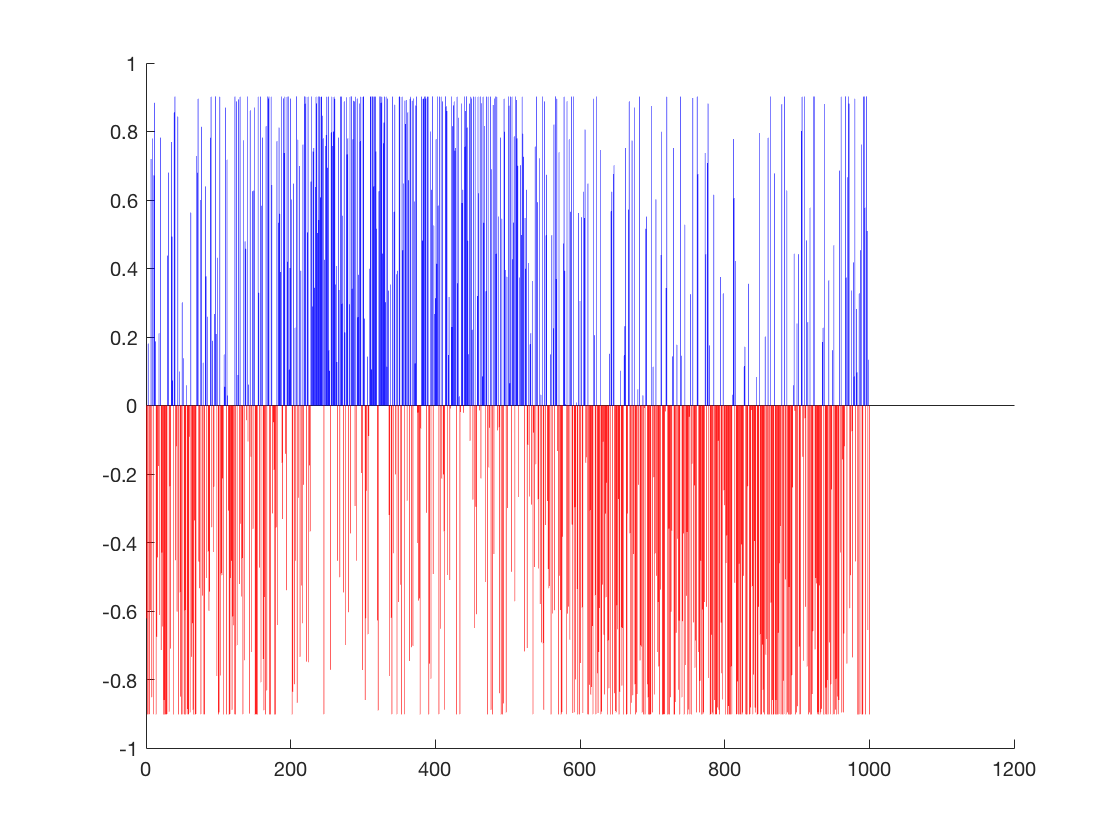
\includegraphics[width=\linewidth]{graphics/moons/centered_untruncated/final_avg.png}
    \end{minipage} \hfill
    \begin{minipage}{0.48\textwidth}
        \centering
        \caption{\label{fig:moon_untruncated_scatter} Without truncation, final clustering obtained. Colored diamonds indicate the labeled nodes.}
        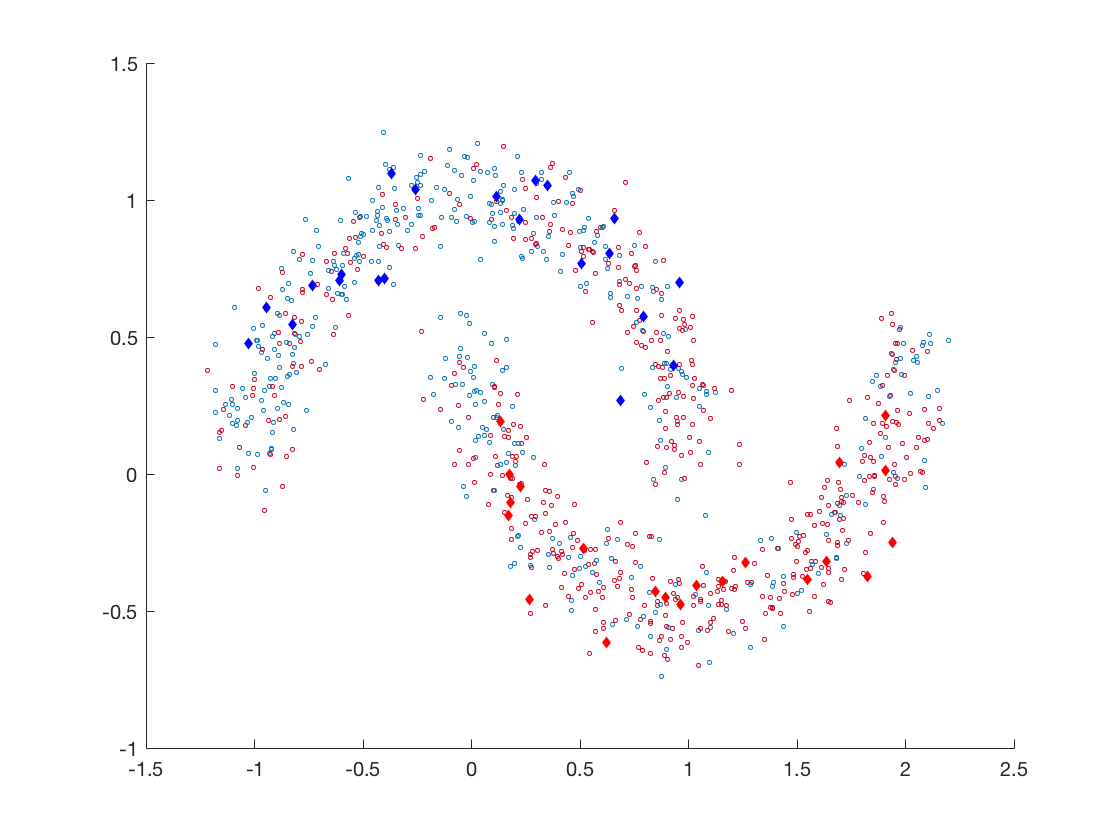
\includegraphics[width=\linewidth]{graphics/moons/centered_untruncated/final_scatter.png}
    \end{minipage}
\end{figure}

Truncating to $M=50$ eigenvectors greatly improved classification and mixing of the hyperparameters. See \cref{fig:moon_truncated_tau}, \cref{fig:moon_truncated_alpha}, \cref{fig:moon_truncated_avg}, \cref{fig:moon_truncated_scatter}.

\begin{figure}[!htb]
    \begin{minipage}{0.48\textwidth}
        \centering
        \caption{\label{fig:moon_truncated_tau} Truncated, $\tau$ trace}
        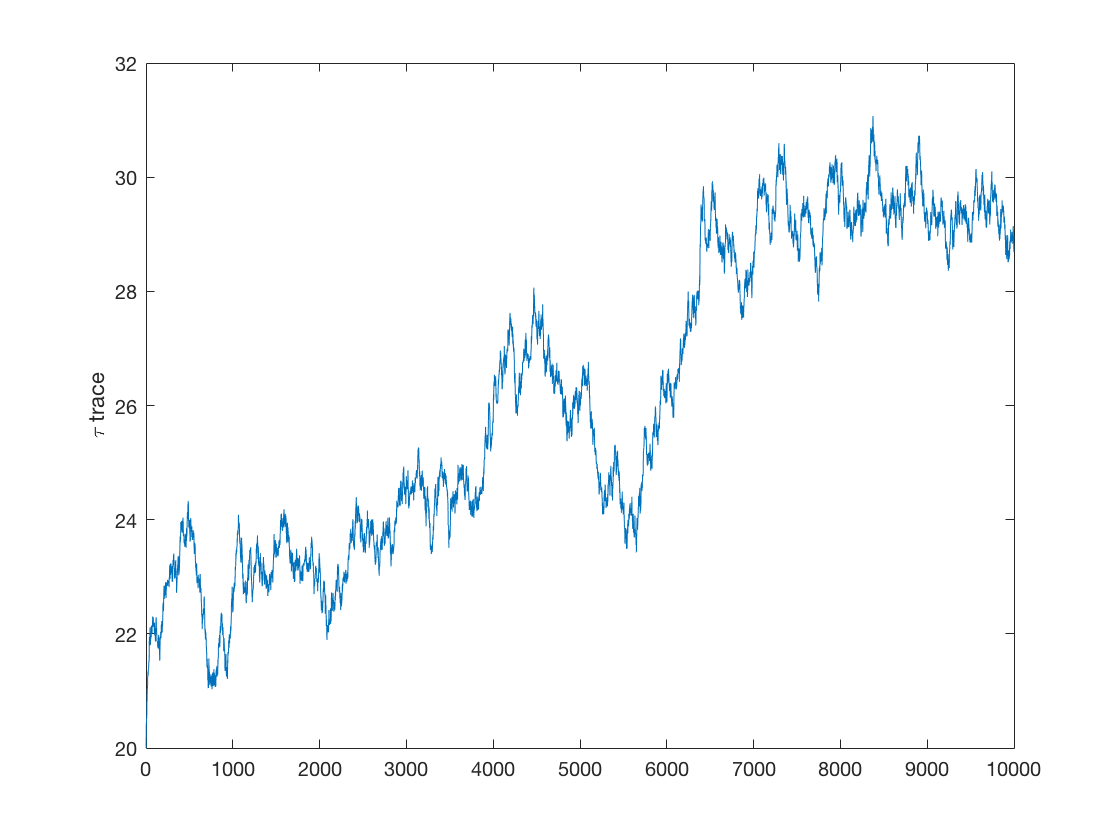
\includegraphics[width=\linewidth]{graphics/moons/centered_truncated/trace_tau.png}
    \end{minipage} \hfill
    \begin{minipage}{0.48\textwidth}
        \centering
        \caption{\label{fig:moon_truncated_alpha} Truncated, $\alpha$ trace}
        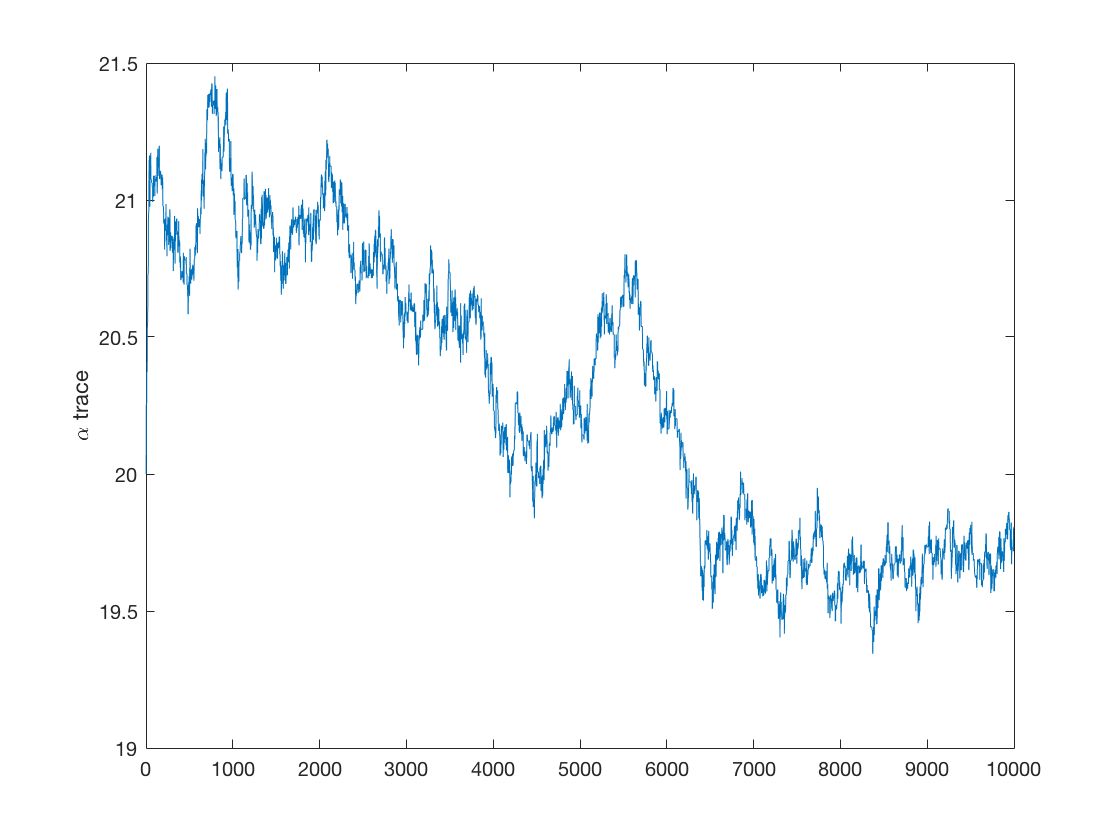
\includegraphics[width=\linewidth]{graphics/moons/centered_truncated/trace_alpha.png}
    \end{minipage}
\end{figure}
\begin{figure}[!htb]
    \begin{minipage}{0.48\textwidth}
        \centering
        \caption{\label{fig:moon_truncated_avg} Truncated, average eigenfunction $u$}
        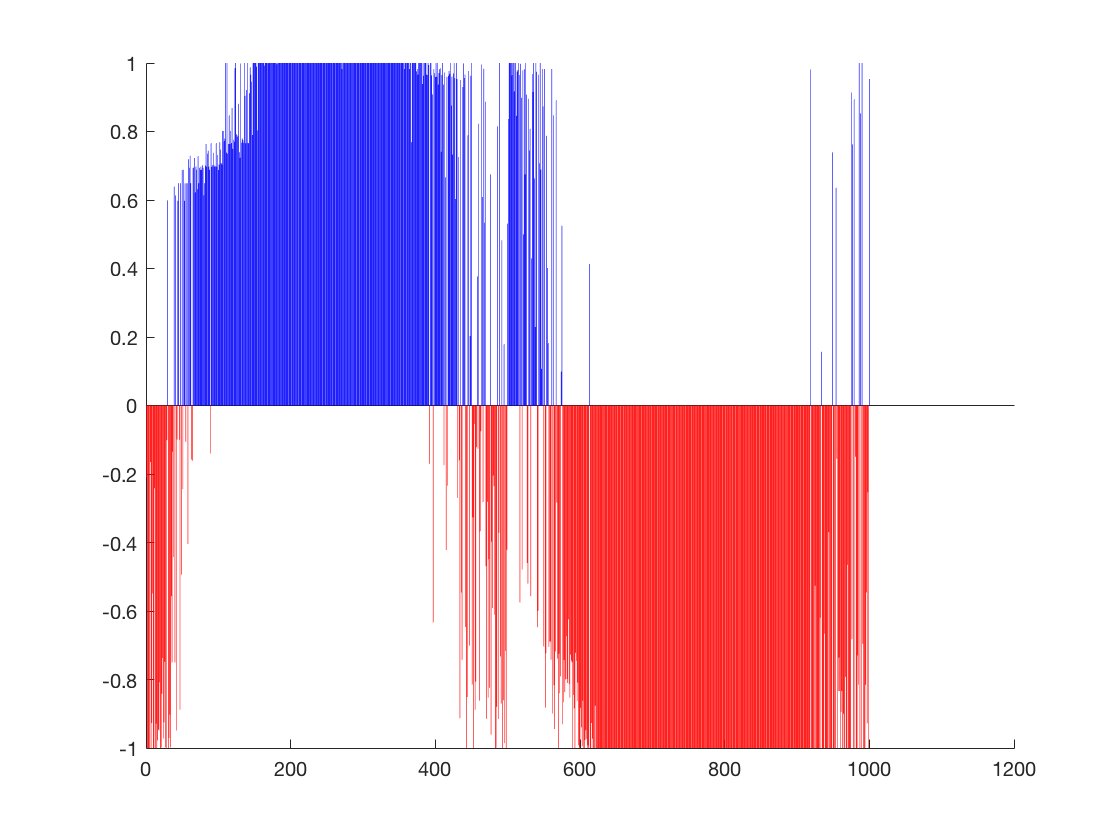
\includegraphics[width=\linewidth]{graphics/moons/centered_truncated/final_avg.png}
    \end{minipage} \hfill
    \begin{minipage}{0.48\textwidth}
        \centering
        \caption{\label{fig:moon_truncated_scatter} Truncated, final clustering obtained}
        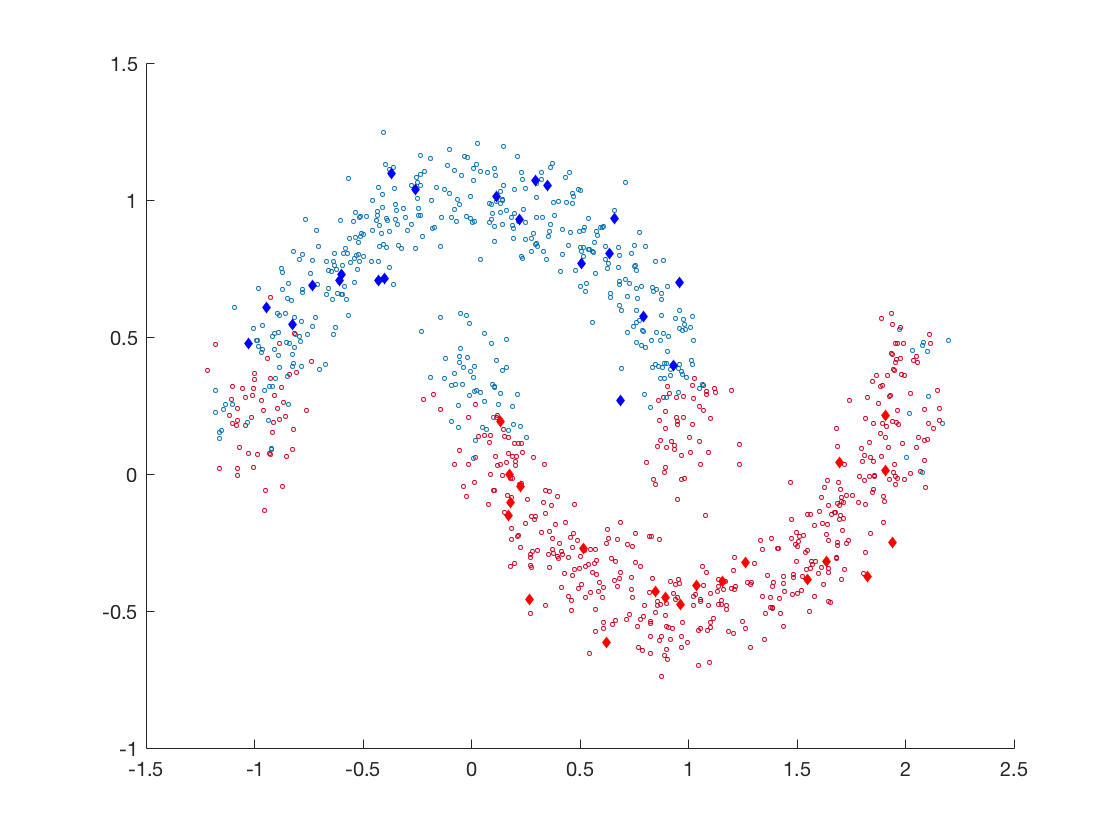
\includegraphics[width=\linewidth]{graphics/moons/centered_truncated/final_scatter.png}
    \end{minipage}
\end{figure}
\subsection{Non-centered parameterization}
Working with the non-centered parameterization, we see that spectral projection/truncating has similar effects when using the unnormalized Laplacian: the algorithm has difficulty clustering the two moons without truncation, and is able to cluster when truncating to $M=50$ eigenvectors, with an accuracy of about $80\%$. See \cref{fig:moon_noncentered_truncated_tau}, \cref{fig:moon_noncentered_truncated_alpha}, \cref{fig:moon_noncentered_truncated_avg}, \cref{fig:moon_noncentered_truncated_scatter}.

\begin{figure}[!htb]
    \begin{minipage}{0.48\textwidth}
        \centering
        \caption{\label{fig:moon_noncentered_truncated_tau} Noncentered truncated, $\tau$ trace}
        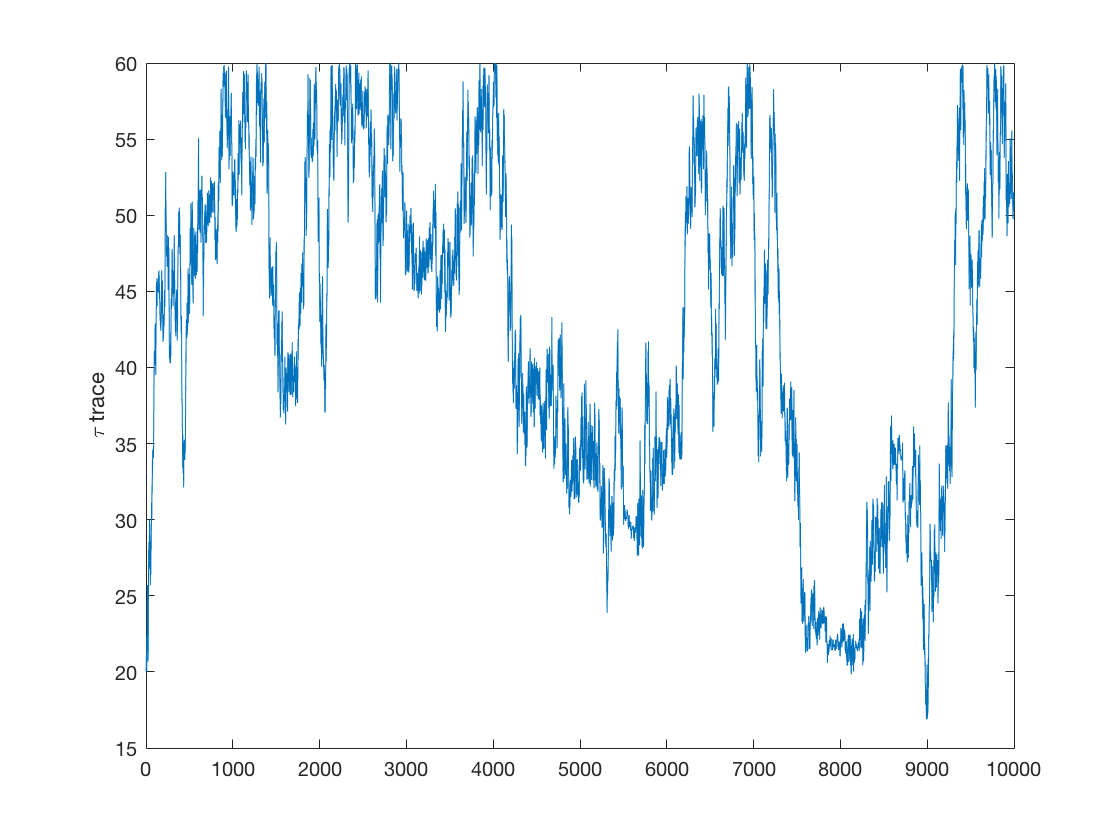
\includegraphics[width=\linewidth]{graphics/moons/noncentered_un_truncated/trace_tau.png}
    \end{minipage} \hfill
    \begin{minipage}{0.48\textwidth}
        \centering
        \caption{\label{fig:moon_noncentered_truncated_alpha} Noncentered truncated, $\alpha$ trace}
        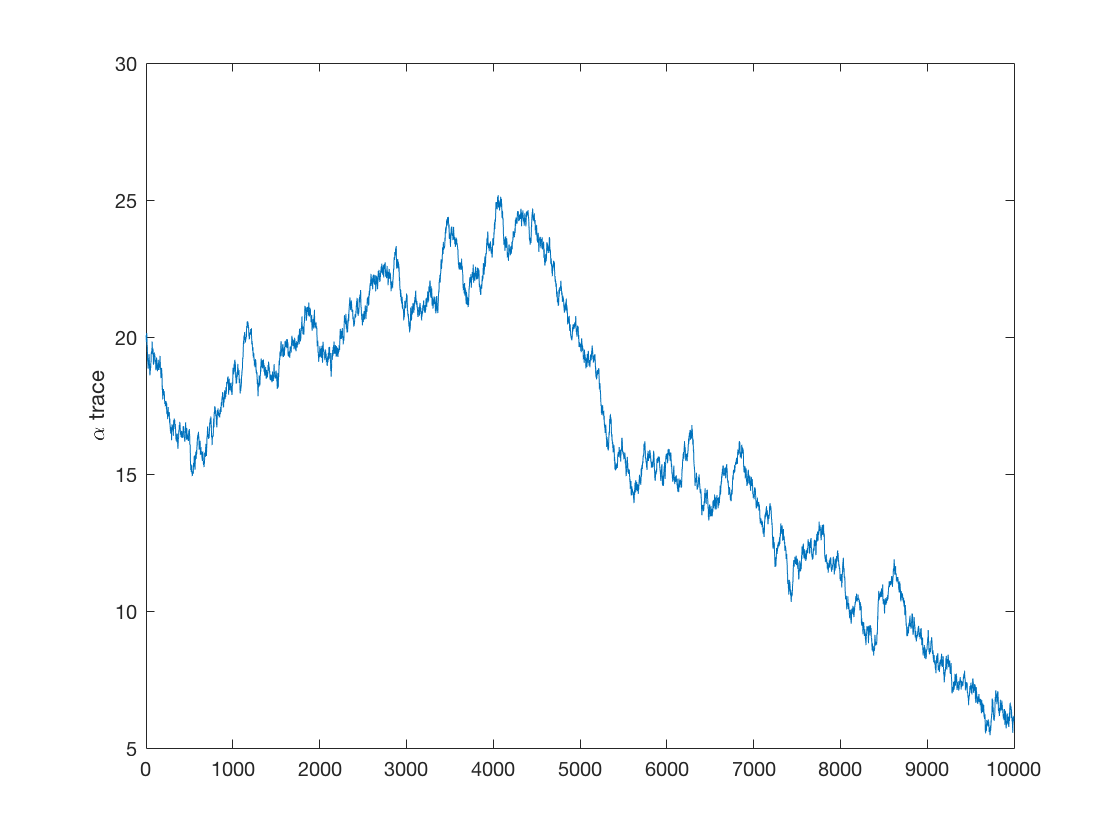
\includegraphics[width=\linewidth]{graphics/moons/noncentered_un_truncated/trace_alpha.png}
    \end{minipage}
\end{figure}
\begin{figure}[!htb]
    \begin{minipage}{0.48\textwidth}
        \centering
        \caption{\label{fig:moon_noncentered_truncated_avg} Noncentered truncated, average eigenfunction $u$}
        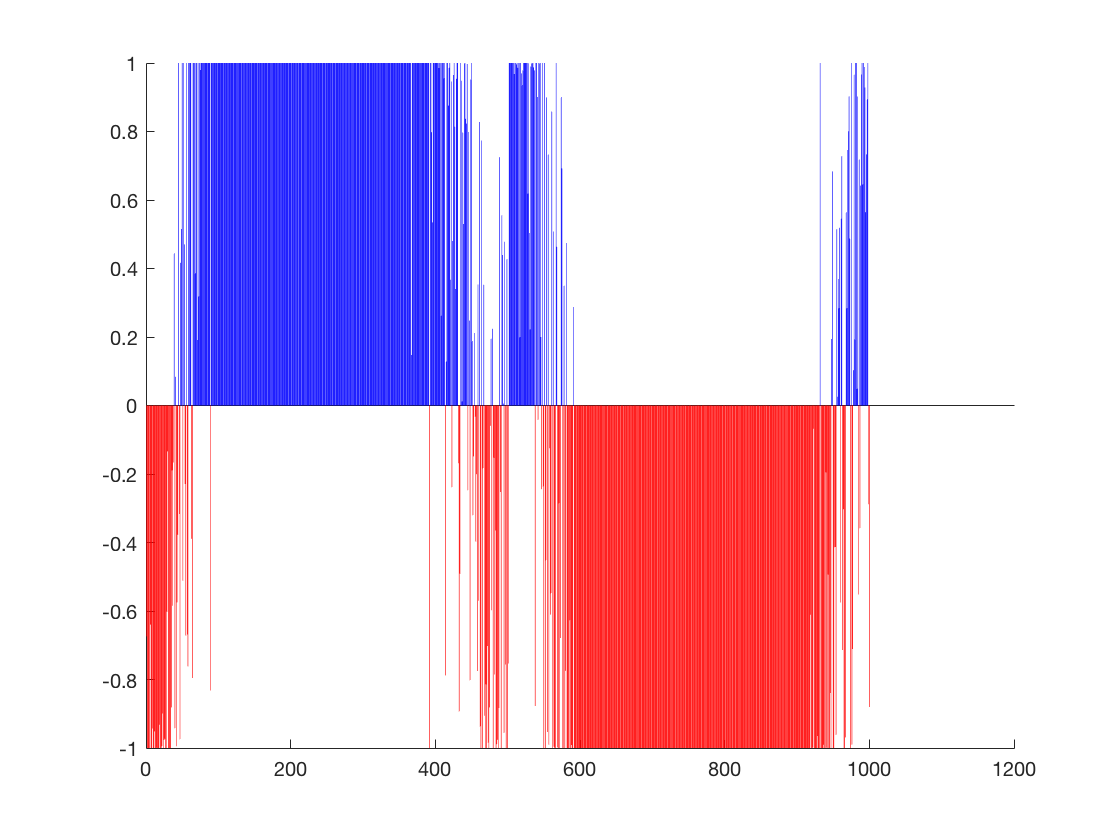
\includegraphics[width=\linewidth]{graphics/moons/noncentered_un_truncated/final_avg.png}
    \end{minipage} \hfill
    \begin{minipage}{0.48\textwidth}
        \centering
        \caption{\label{fig:moon_noncentered_truncated_scatter} Noncentered truncated, final clustering obtained}
        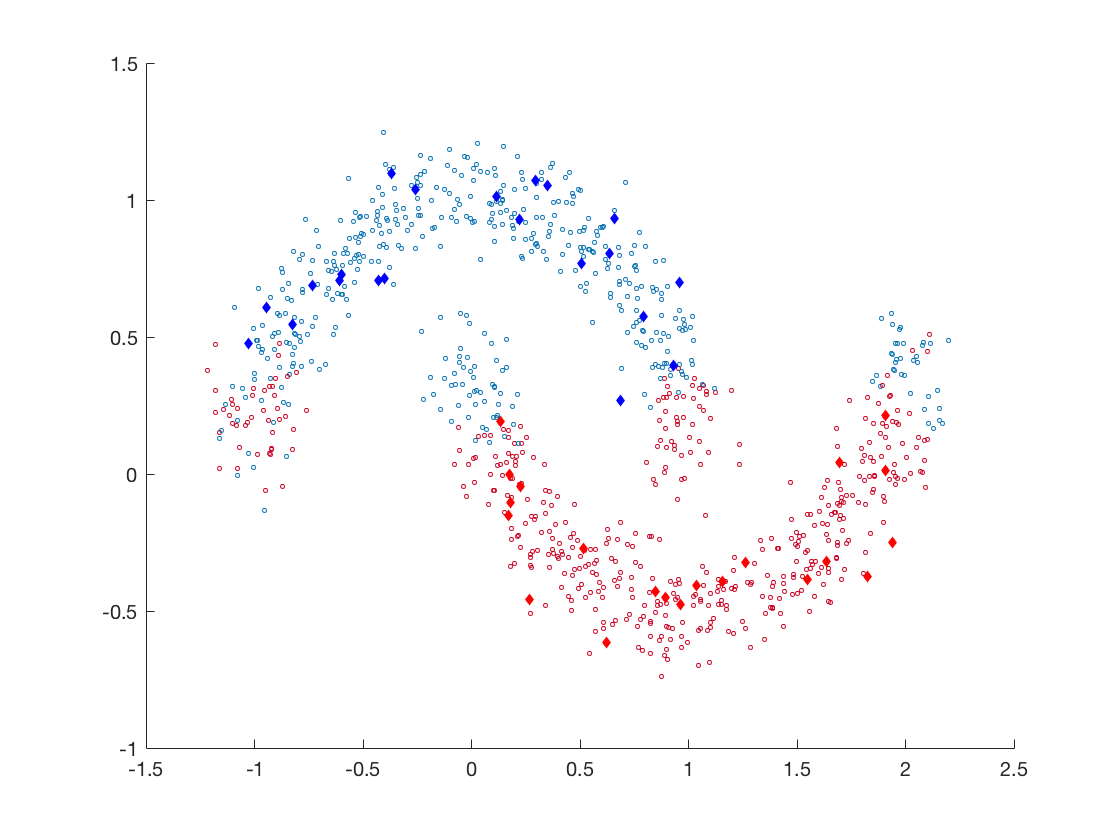
\includegraphics[width=\linewidth]{graphics/moons/noncentered_un_truncated/final_scatter.png}
    \end{minipage}
\end{figure}


However, we get better results with the non-centered parameterization when using the self-tuning unnormalized Laplacian. It seems that the self-tuning Laplacian offers more clustering information in its higher order eigenvectors, while the eigenvectors beyond the Fiedler vector in the unnormalized Laplacian are less useful. Refer to \cref{fig:moon_laplacian_un}, \cref{fig:moon_laplacian_selftuning}. Clustering accuracy is around $98\%$. See \cref{fig:noncentered_selftuning_tau}, \cref{fig:noncentered_selftuning_alpha}, \cref{fig:noncentered_selftuning_avg}, \cref{fig:noncentered_selftuning_scatter}.

\begin{figure}[!htb]
    \begin{minipage}{0.48\textwidth}
        \centering
        \caption{\label{fig:moon_laplacian_un} First eigenvectors of unnormalized Laplacian for intertwined moons data}
        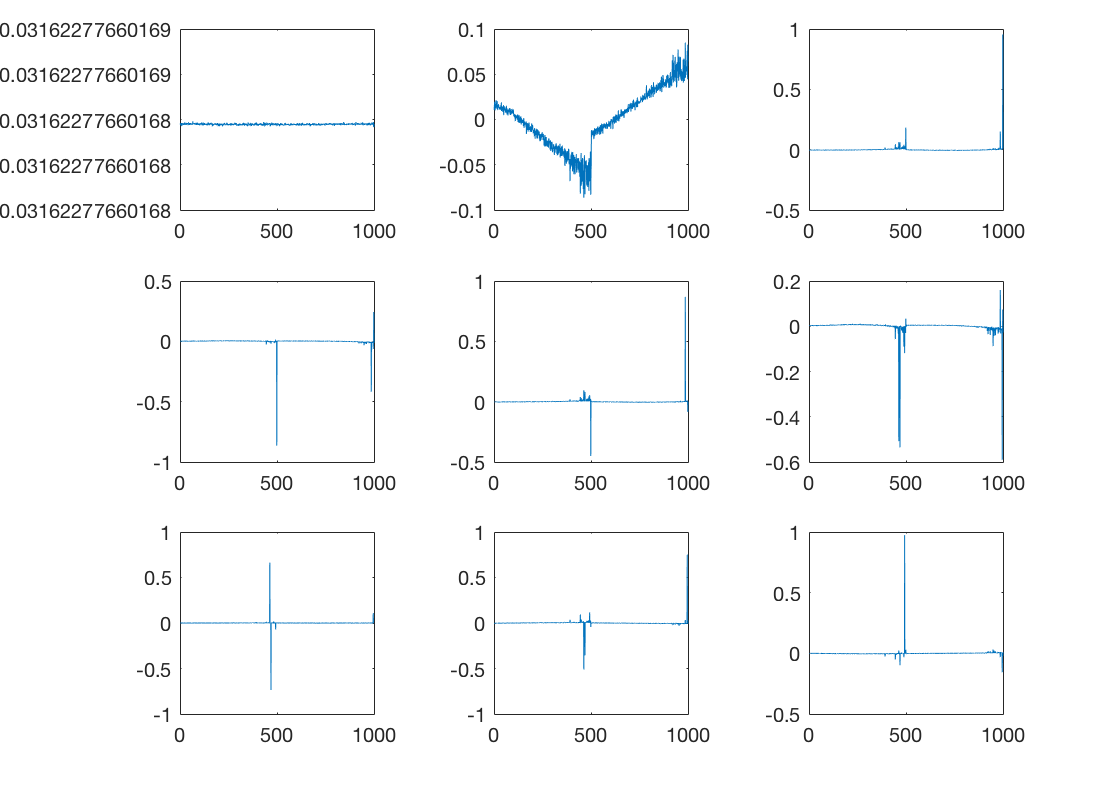
\includegraphics[width=\linewidth]{graphics/moon_laplacian_un.png}
    \end{minipage} \hfill
    \begin{minipage}{0.48\textwidth}
        \centering
        \caption{\label{fig:moon_laplacian_selftuning} First eigenvectors of unnormalized self-tuning Laplacian for intertwined moons data}
        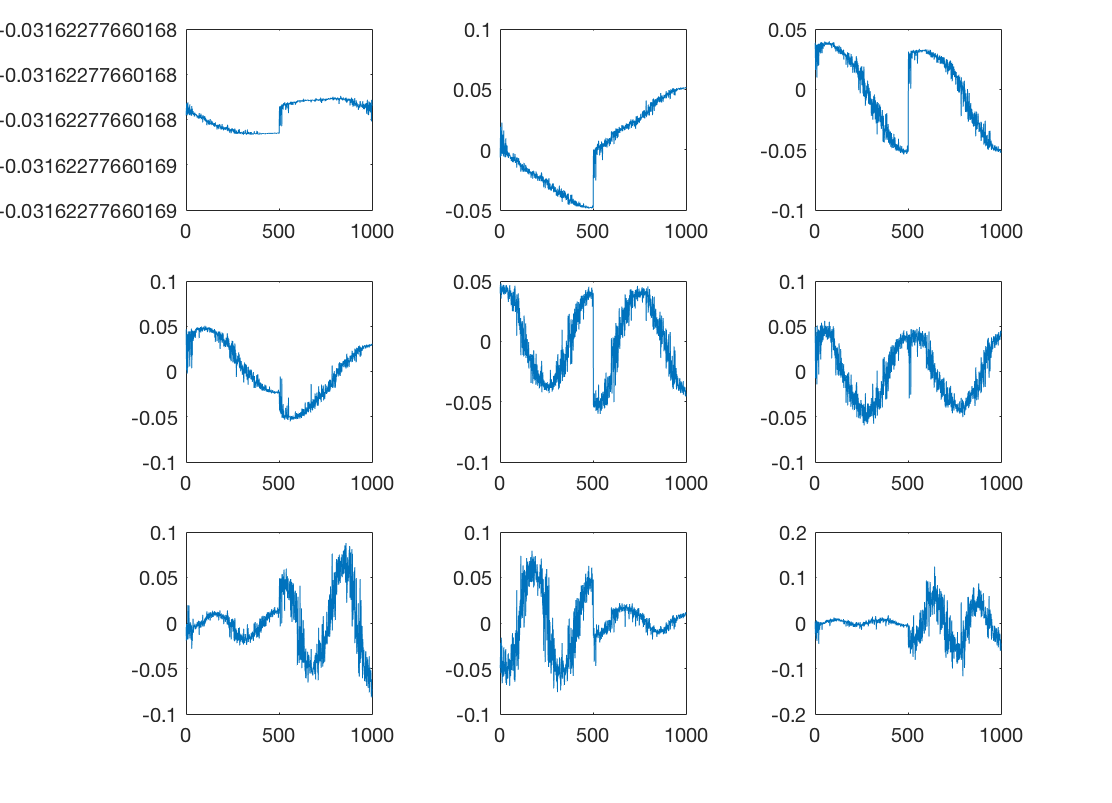
\includegraphics[width=\linewidth]{graphics/moon_laplacian_selftuning.png}
    \end{minipage}
\end{figure}

\begin{figure}[!htb]
    \begin{minipage}{0.48\textwidth}
        \centering
        \caption{\label{fig:noncentered_selftuning_tau} Self tuning, $\tau$ trace}
        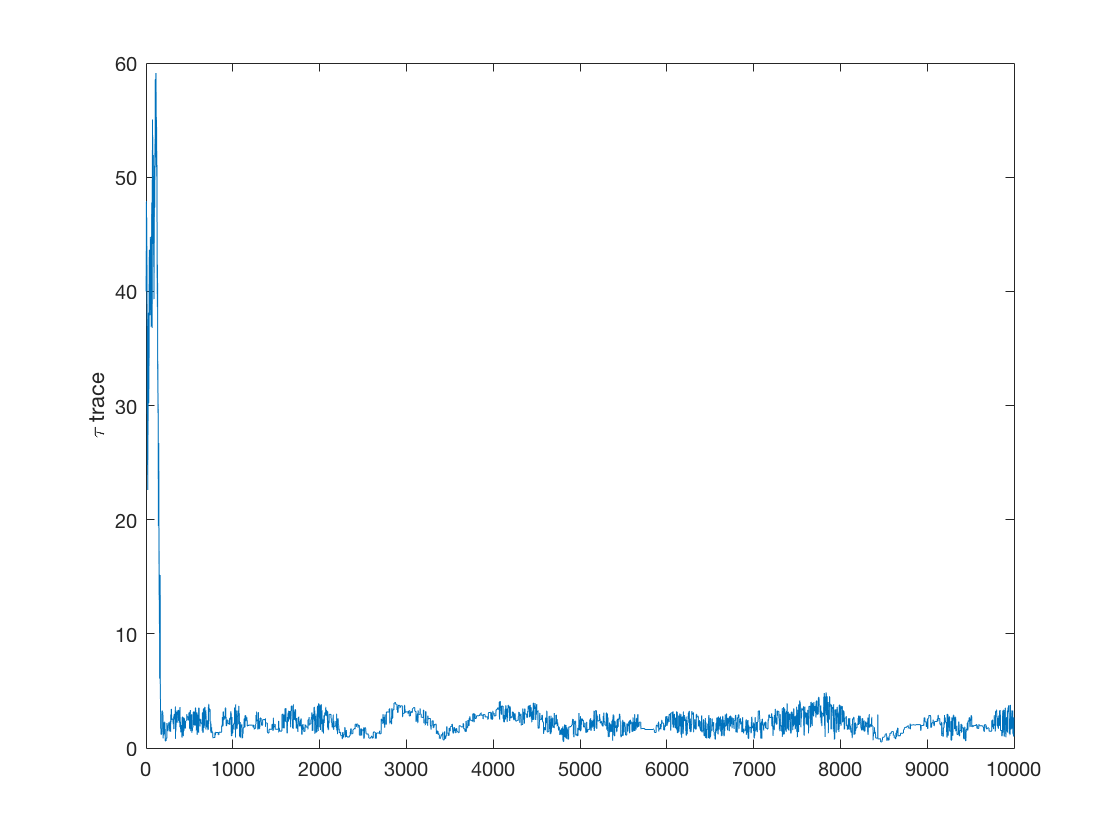
\includegraphics[width=\linewidth]{graphics/moons/noncentered_selftuning/trace_tau.png}
    \end{minipage} \hfill
    \begin{minipage}{0.48\textwidth}
        \centering
        \caption{\label{fig:noncentered_selftuning_alpha} Self tuning, $\alpha$ trace}
        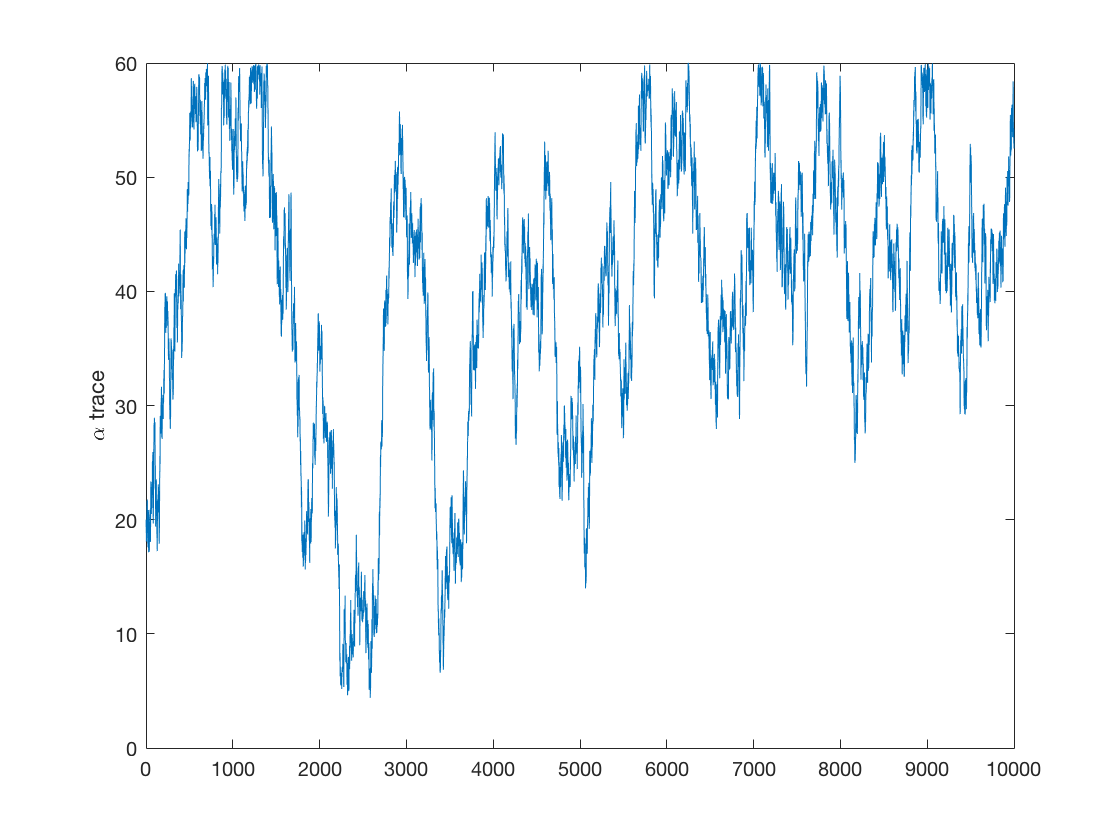
\includegraphics[width=\linewidth]{graphics/moons/noncentered_selftuning/trace_alpha.png}
    \end{minipage}
\end{figure}
\begin{figure}[!htb]
    \begin{minipage}{0.48\textwidth}
        \centering
        \caption{\label{fig:noncentered_selftuning_avg} Self tuning, average eigenfunction $u$}
        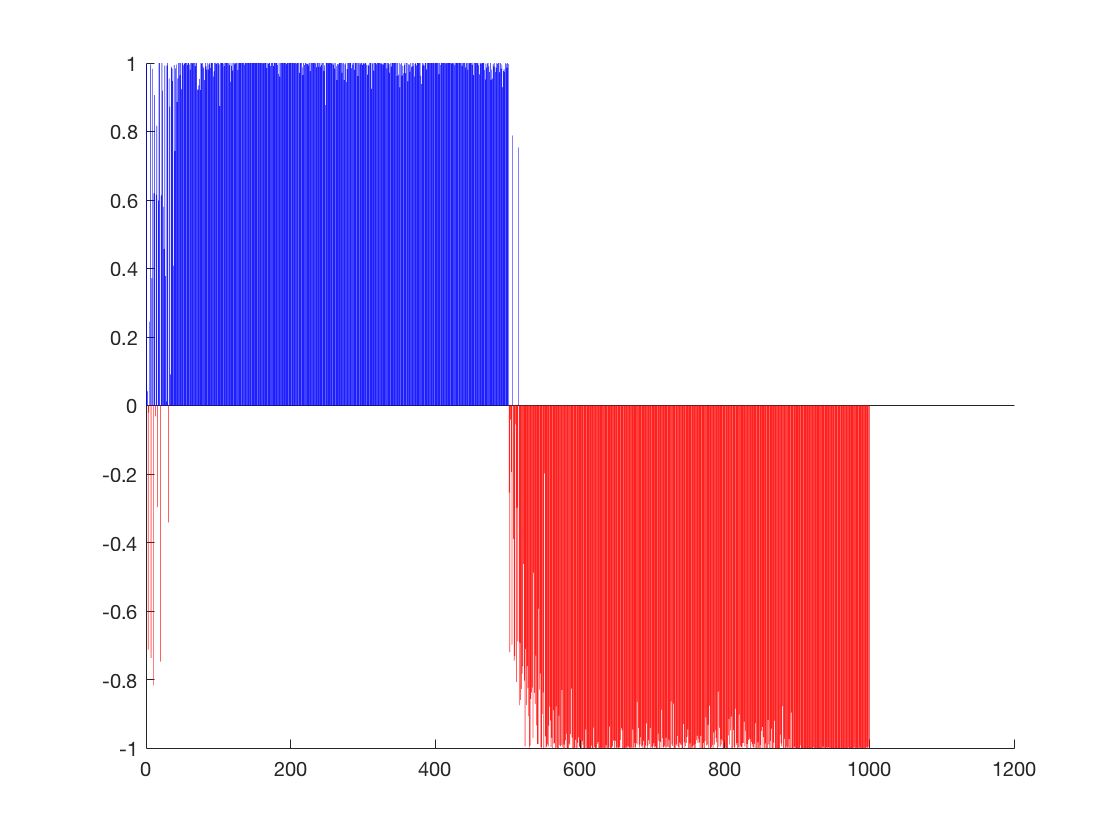
\includegraphics[width=\linewidth]{graphics/moons/noncentered_selftuning/final_avg.png}
    \end{minipage} \hfill
    \begin{minipage}{0.48\textwidth}
        \centering
        \caption{\label{fig:noncentered_selftuning_scatter} Self tuning, clustering obtained}
        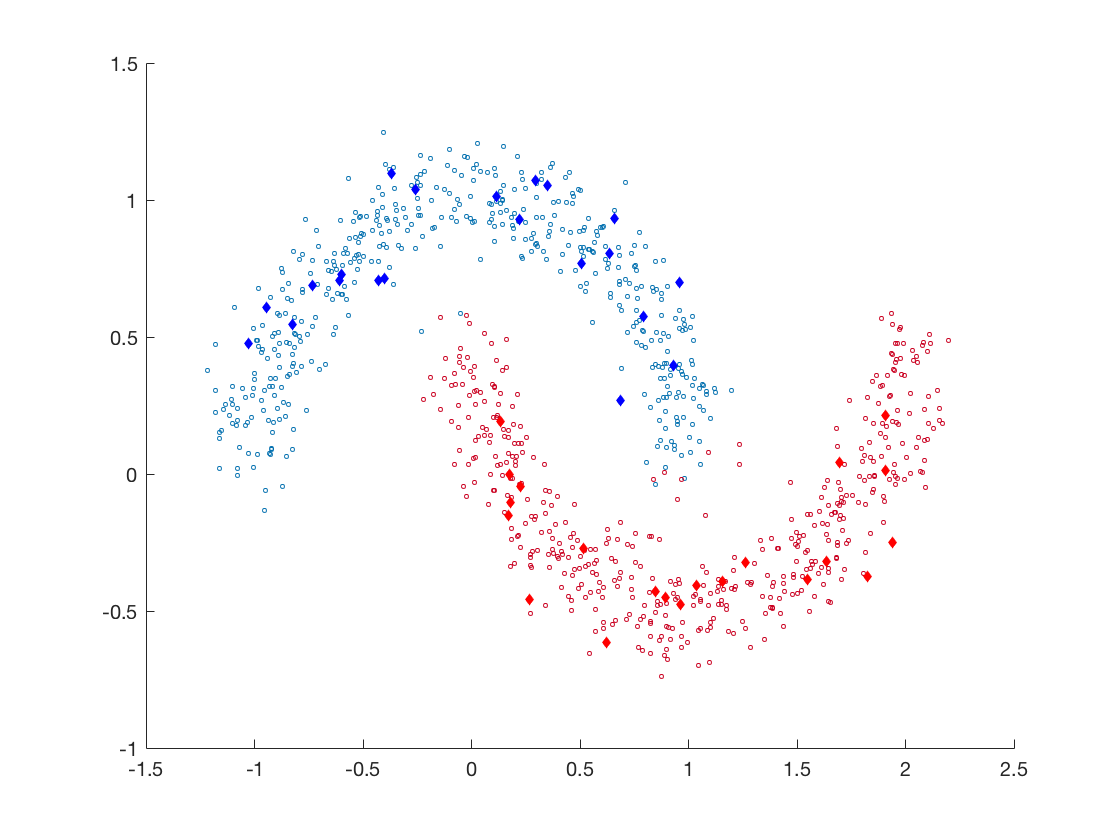
\includegraphics[width=\linewidth]{graphics/moons/noncentered_selftuning/final_scatter.png}
    \end{minipage}
\end{figure}
\end{document}